\section{Sequence Imminece}{\label{sec:sequences}}
\begin{topics}
\verb!array! traversal, manipulation and previous sections.
\end{topics}
\begin{note}
	This is the last problem set where we use Simplecpp. We will move onto C++ from the next problem set.
\end{note}
\subsection{Josephus Problem}
Suppose there are $n$ terrorists around a circle facing towards the centre. They are numbered $1$ to $n$ along clockwise direction. Initially, terrorist 1 has the sword. Now, the terrorist with sword kills the $k$\textsuperscript{th} nearest alive terrorist to its left and passes the sword to $(k+1)$\textsuperscript{st} nearest alive terrorist to its left. The process repeats. Basically, every $k$\textsuperscript{th} terrorist is killed until only one survives. Then the last terrorist is killed.
\begin{figure}[H]
    \centering
    
\includegraphics[width = 0.15\linewidth]{Josephus.pdf}
    \caption{Example arrangement of 10 terrorists}
    \label{fig:jp}
\end{figure}
\vspace{-1.5em}
For example, in the above arrangement,\\
when $k=1,$ 1 kills 2, 3 kills 4, 5 kills 6, 7 kills 8, 9 kills 10, 1 kills 3, 5 kills 7, 9 kills 1 and 5 kills 9. So, 5 survives;\\% and is killed last;\\
when $k=2,$ 1 kills 3, 4 kills 6, 7 kills 9, 10 kills 2, 4 kills 7, 8 kills 1, 4 kills 8, 10 kills 5 and 4 kills 10. So, 4 survives.\\% and is killed last.
\textbf{Problem Statement:}\\
For a given $n, k$ pair, and starting position $1$, print the terrorists in the order they are killed.
\begin{testcases}
	{$t$ \hfill(number of test cases, an integer)\\
	$n_1\ k_1\ \quad n_2\ k_2\ \quad \ldots\quad n_t\ k_t$ \hfill($t$ space seperated pairs (number of terrorists $n$ and $k$) for each testcase)}
	{Terrorists in the order they are killed \hfill(each test case on a newline)}
	{$1 \leq k_i \leq n_i \leq 100$}
	{9\\1 1\quad2 1\quad4 1\quad4 2\quad8 1\quad8 3\quad10 2\quad16 7\quad50 25}
	{1\\2 1\\2 4 3 1\\3 2 4 1\\2 4 6 8 3 7 5 1\\4 8 5 2 1 3 7 6\\3 6 9 2 7 1 8 5 10 4\\8 16 9 2 12 6 3 15 14 1 5 11 10 4 13 7\\26 2 29 6 34 12 41 20 50 32 14 46 30 15 49 37 23 11 3 43 36 28 24 21 19 22 27 35 42 1 10 33 4 25 7 44 38 31 40 5 18 16 39 9 17 45 48 13 8 47}
	{https://github.com/paramrathour/CS-101/tree/main/Starter Codes/Josephus Problem.cpp}
\end{testcases}
\begin{note}
	Verify your program on even more testcases from \href{https://cses.fi/problemset/task/2163/}{here}.
\end{note}
\begin{funvideo}
	\href{https://youtu.be/uCsD3ZGzMgE}{The Josephus Problem -- Numberphile}
\end{funvideo}
\subsection{Van Eck's Sequence}
The Van Eck's Sequence is defined as follows:

$a_0 = 0$ then for $n>0$,\\
$a_{n+1} = n-m$, where $m$ is the maximal index $<n$ such that $a_{m}=a_{n}$.
\\If such $m<n$ doesn't exist, then we take $m=n\ \rightarrow\ a_{n+1}=0$.

\textbf{Problem Statement:}\\
Generate the first $n+1$ elements $a_0,a_1,\ldots,a_n$ of the Van Eck's Sequence.
\begin{testcasesMore}
	{$n$ \hfill(a single integer)}
	{$a_0\ a_1\ \ldots\ a_n$\hfill(space seperated integers)}
	{$1 \leq n \leq 100000$}
	{500}
	{0 0 1 0 2 0 2 2 1 6 0 5 0 2 6 5 4 0 5 3 0 3 2 9 0 4 9 3 6 14 0 6 3 5 15 0 5 3 5 2 17 0 6 11 0 3 8 0 3 3 1 42 0 5 15 20 0 4 32 0 3 11 18 0 4 7 0 3 7 3 2 31 0 6 31 3 6 3 2 8 33 0 9 56 0 3 8 7 19 0 5 37 0 3 8 8 1 46 0 6 23 0 3 9 21 0 4 42 56 25 0 5 21 8 18 52 0 6 18 4 13 0 5 11 62 0 4 7 40 0 4 4 1 36 0 5 13 16 0 4 8 27 0 4 4 1 13 10 0 6 32 92 0 4 9 51 0 4 4 1 14 131 0 6 14 4 7 39 0 6 6 1 12 0 5 39 8 36 44 0 6 10 34 0 4 19 97 0 4 4 1 19 6 12 21 82 0 9 43 0 3 98 0 3 3 1 15 152 0 6 17 170 0 4 24 0 3 12 24 4 6 11 98 21 29 0 10 45 0 3 13 84 0 4 14 70 0 4 4 1 34 58 0 6 23 144 0 4 9 51 94 0 5 78 0 3 26 0 3 3 1 21 38 0 6 21 4 19 76 0 6 6 1 12 56 166 0 7 111 0 3 21 16 145 0 5 33 206 0 4 23 46 194 0 5 9 47 0 4 9 4 2 223 0 6 33 19 39 132 0 6 6 1 40 185 0 6 5 23 28 0 5 4 22 0 4 3 46 36 151 0 6 15 126 0 4 10 110 0 4 4 1 29 118 0 6 14 112 0 4 9 51 102 0 5 33 50 0 4 9 9 1 20 307 0 7 88 0 3 42 262 0 4 14 27 233 0 5 23 60 0 4 9 22 60 5 8 210 0 8 3 22 8 3 3 1 34 156 0 10 63 0 3 8 11 183 0 5 22 17 199 0 5 5 1 19 109 0 6 73 0 3 19 7 58 183 20 64 0 8 26 174 0 4 52 319 0 4 4 1 25 331 0 6 25 4 7 23 69 0 7 4 6 9 71 0 6 4 6 2 158 0 6 4 6 2 6 2 2 1 30 0 10 73 54 0 4 13 247 0 4 4 1 13 6 18 367 0 8 59 0 3 70 257 0 4 14 123 0 4 4}
	{https://github.com/paramrathour/CS-101/tree/main/Test Cases/Van Eck's Sequence/Input.txt}
	{https://github.com/paramrathour/CS-101/tree/main/Test Cases/Van Eck's Sequence/Output.txt}
	{https://github.com/paramrathour/CS-101/tree/main/Starter Codes/Van Eck's Sequence.cpp}
\end{testcasesMore}
\begin{funvideo}
	\href{https://youtu.be/etMJxB-igrc}{Don't Know (the Van Eck Sequence) -- Numberphile}
\end{funvideo}
\subsection{Look-And-Say Sequence}
As the name suggests, the look-and-say sequence is generated by the \emph{reading} of the digits of the previous sequence.\\% in a \emph{look-and-say manner}.\\
For example, starting with the sequence \textbf{1}.
\begin{itemize}
\item \textbf{1} is read off as "one 1" or \textbf{11}.
\item \textbf{11} is read off as "two 1s" or \textbf{21}.
\item \textbf{21} is read off as "one 2, one 1" or \textbf{1211}.
\item \textbf{1211} is read off as "one 1, one 2, two 1s" or \textbf{111221}.
\item \textbf{111221} is read off as "three 1s, two 2s, one 1" or \textbf{312211} and so on.
\end{itemize}
\textbf{Problem Statement:}\\
Generate the first $n$ iterations of the look-and-say sequence.
\begin{testcasesMore}
	{$n$ \hfill(a single integer)}
	{First $n$ iterations of the look-and-say sequence\hfill(each iteration on a newline)}
	{$1 \leq n_i \leq 40$}
	{15}
	{1\\[0.5em]11\\[0.5em]21\\[0.5em]1211\\[0.5em]111221\\[0.5em]312211\\[0.5em]13112221\\[0.5em]1113213211\\[0.5em]31131211131221\\[0.5em]13211311123113112211\\[0.5em]11131221133112132113212221\\[0.5em]3113112221232112111312211312113211\\[0.5em]1321132132111213122112311311222113111221131221\\[0.5em]11131221131211131231121113112221121321132132211331222113112211\\[0.5em]311311222113111231131112132112311321322112111312211312111322212311322113212221}
	{https://github.com/paramrathour/CS-101/tree/main/Test Cases/Look-And-Say Sequence/Input.txt}
	{https://github.com/paramrathour/CS-101/tree/main/Test Cases/Look-And-Say Sequence/Output.txt}
	{https://github.com/paramrathour/CS-101/tree/main/Starter Codes/Look-And-Say Sequence.cpp}
\end{testcasesMore}
\begin{funvideo}
	\href{https://youtu.be/ea7lJkEhytA}{Look-and-Say Numbers (feat John Conway) -- Numberphile}
\end{funvideo}
\KOMAoptions{paper=A3}
\recalctypearea
\subsection{Thue-Morse Sequence}{\label{pp:thuemorsesequence}}
Thue-Morse Sequence aka Fair Share Sequence is an infinite binary sequence obtained by starting with 0 and successively appending the Boolean complement of the sequence obtained thus far (called prefixes of the sequence).\\
For example, starting with the sequence \textbf{0},
\begin{itemize}
	\item Append complement of \textbf{0}, we get 0\textbf{1}
	\item Append complement of \textbf{01}, we get 01\textbf{10}
	\item Append complement of \textbf{0110}, we get 0110\textbf{1001} and so on.
\end{itemize}
Also, by using Thue–Morse sequence elements in the turtle simulator, we get a mysterious curve\footnote{called Koch curve, it is a fractal curve that has infinite length but contained in a finite area. Can you see why?} by following the below rule.
\begin{itemize}
	\item If an element is 0, then the turtle rotates \verb!right! by 180\textdegree.
	\item If an element is 1, then the turtle moves \verb!forward! by one unit and then rotates \verb!right! by 60\textdegree.
\end{itemize}
Can you figure out the pattern of this curve?

\textbf{Problem Statement:}\\
Generate the first $n$ elements of the Thue-Morse sequence and draw the corresponding curve using \verb!turtleSim!.\\
Scale the curve in such a way that it roughly takes same width and height for all $n$.
% \begin{testcasesMore}
% 	{$t$ \hfill(number of test cases, an integer)\\
% 	$n_1\ n_2\ \ldots n_t$ \hfill($t$ space seperated integers for each testcase)}
% 	{First $n_i$ elements of the Thue-Morse sequence and the curve.\hfill(each testcase on a newline)}
% 	{$1 \leq n_i \leq 100000$ ($n_i$ need not be a power of 2)}
% 	{4\\2 32 111 128}
% 	{01\\01101001100101101001011001101001\\011010011001011010010110011010011001011001101001011010011001011010010110011010010110100110010110011010011001011\\01101001100101101001011001101001100101100110100101101001100101101001011001101001011010011001011001101001100101101001011001101001}
% 	{https://github.com/paramrathour/CS-101/tree/main/Test Cases/Thue-Morse Sequence/Input.txt}
% 	{https://github.com/paramrathour/CS-101/tree/main/Test Cases/Thue-Morse Sequence/Output.txt}
% 	{https://github.com/paramrathour/CS-101/tree/main/Starter Codes/Thue-Morse Sequence.cpp}
% \end{testcasesMore}
\begin{testcasesMore}
	{$n$ \hfill(a single integer)}
	{First $n$ elements of the Thue-Morse sequence and the curve.}
	{$1 \leq n \leq 100000$ ($n$ need not be a power of 2)}
	{111}
	{011010011001011010010110011010011001011001101001011010011001011010010110011010010110100110010110011010011001011}
	{https://github.com/paramrathour/CS-101/tree/main/Test Cases/Thue-Morse Sequence/Input.txt}
	{https://github.com/paramrathour/CS-101/tree/main/Test Cases/Thue-Morse Sequence/Output.txt}
	{https://github.com/paramrathour/CS-101/tree/main/Starter Codes/Thue-Morse Sequence.cpp}
\end{testcasesMore}
\textbf{The output Koch Curve convergents}
\begin{figure}[H]
	\centering
	\begin{subfigure}{0.3\linewidth}
		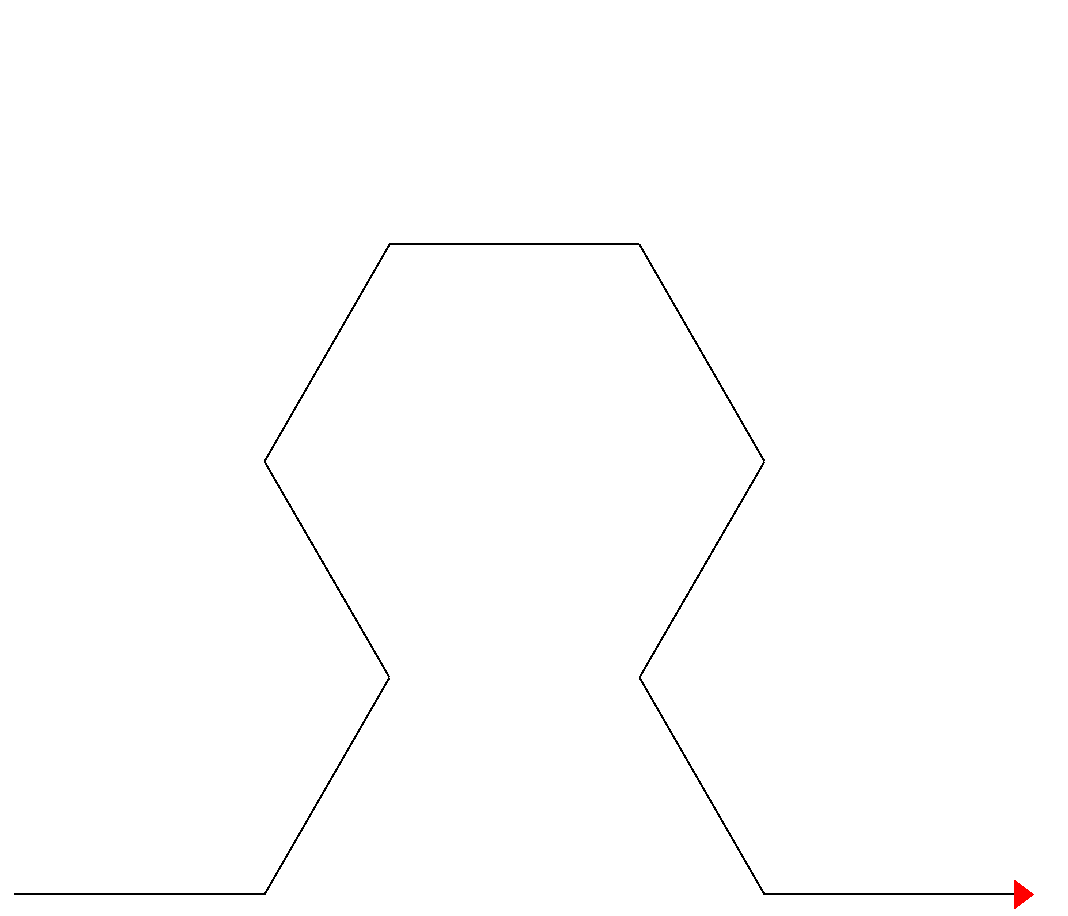
\includegraphics[width = \linewidth]{Thue-Morse Sequence/2.png}
		\caption{Iteration 0, $n=2$}
	\end{subfigure}
	\begin{subfigure}{0.3\linewidth}
		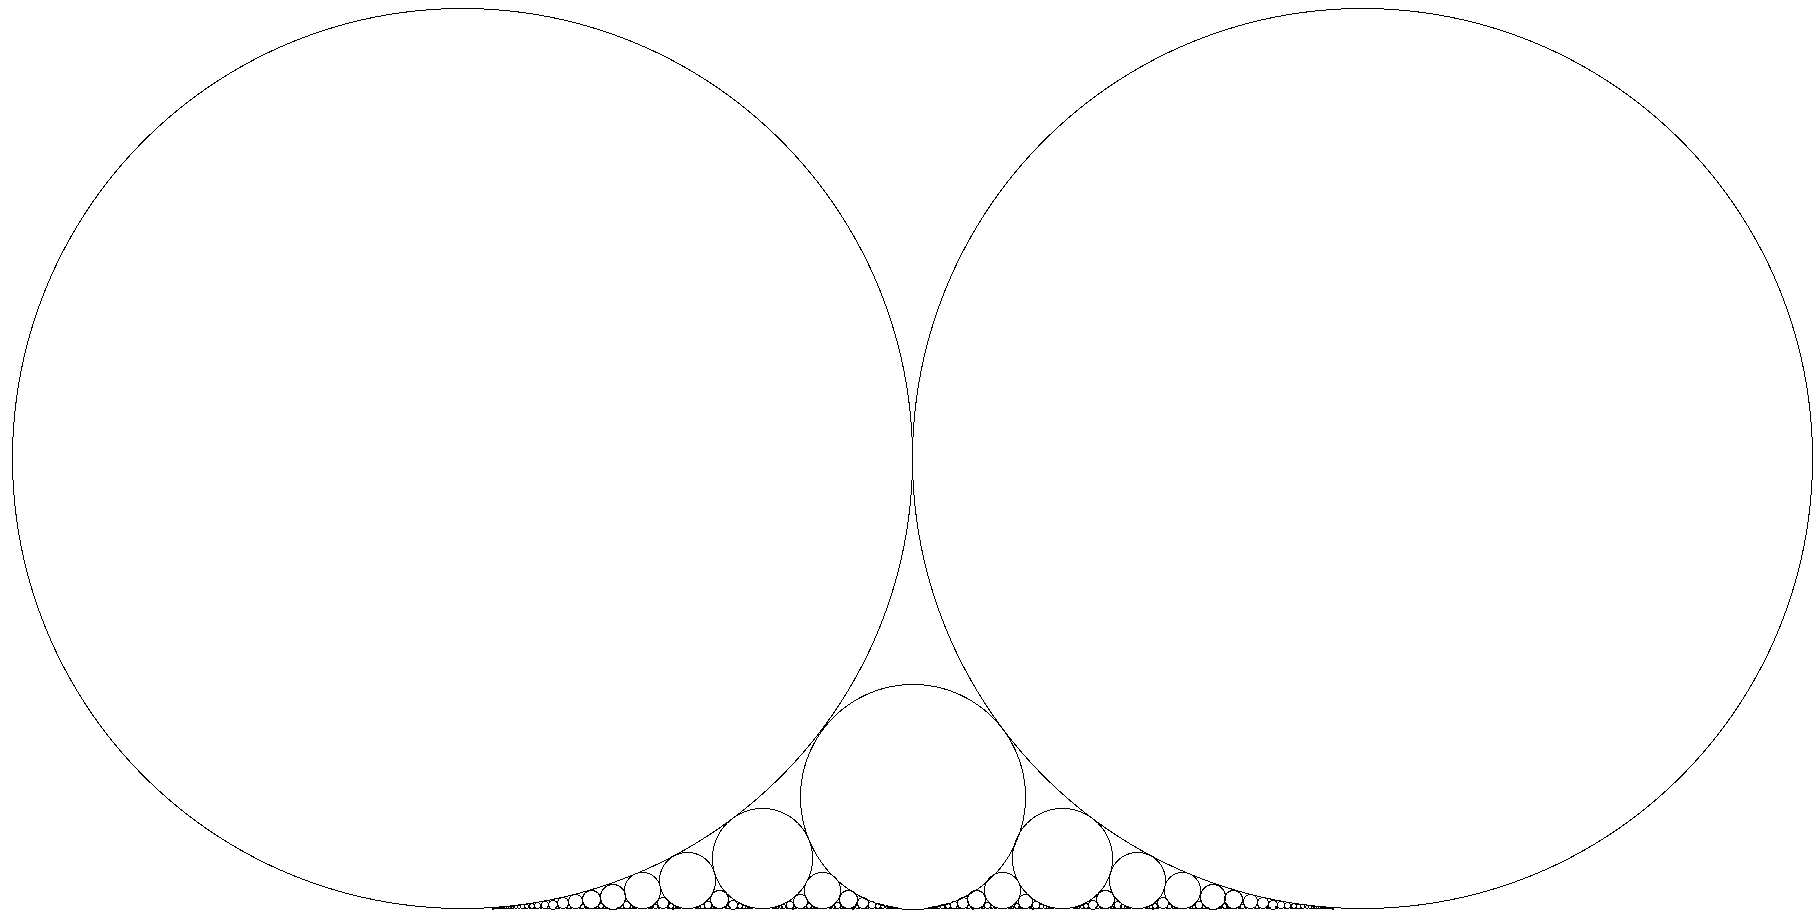
\includegraphics[width = \linewidth]{Thue-Morse Sequence/8.png}
		\caption{Iteration 1, $n=8$}
	\end{subfigure}
	\begin{subfigure}{0.3\linewidth}
		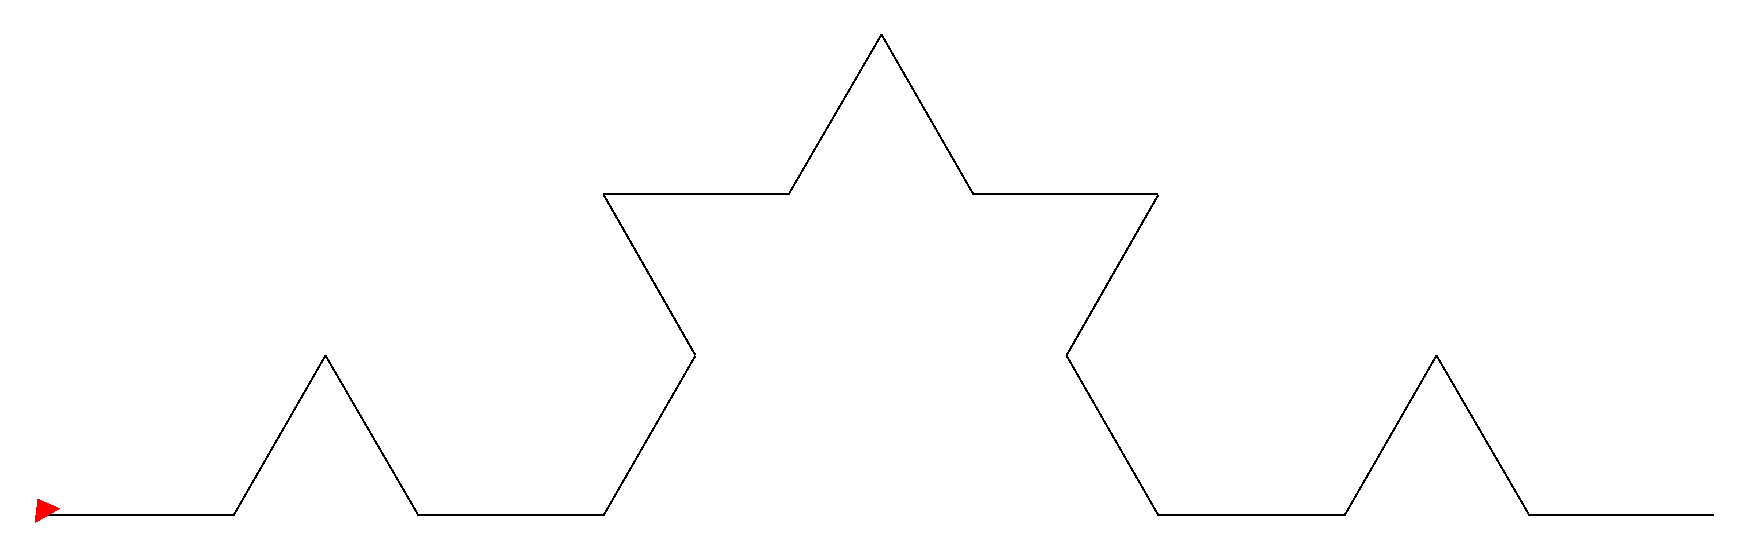
\includegraphics[width = \linewidth]{Thue-Morse Sequence/32.png}
		\caption{Iteration 2, $n=32$}
	\end{subfigure}
	\begin{subfigure}{0.3\linewidth}
		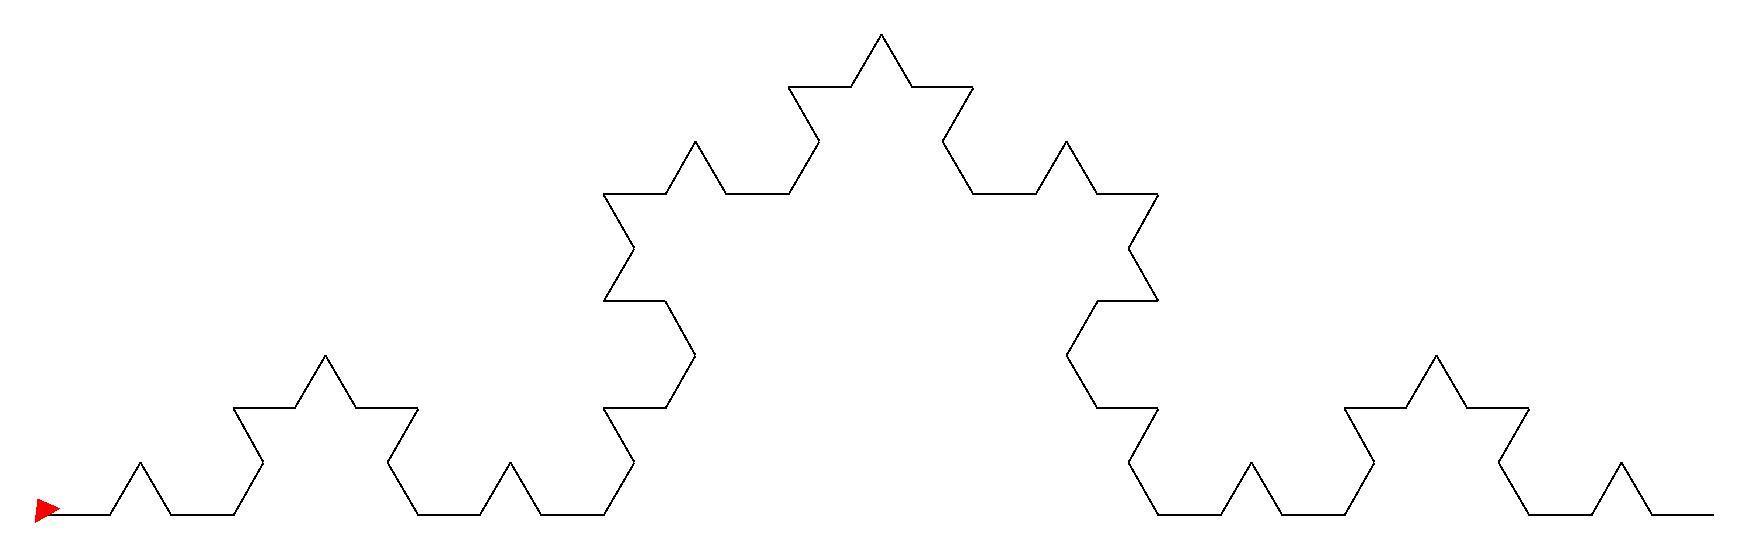
\includegraphics[width = \linewidth]{Thue-Morse Sequence/128.png}
		\caption{Iteration 3, $n=128$}
	\end{subfigure}
	\begin{subfigure}{0.3\linewidth}
		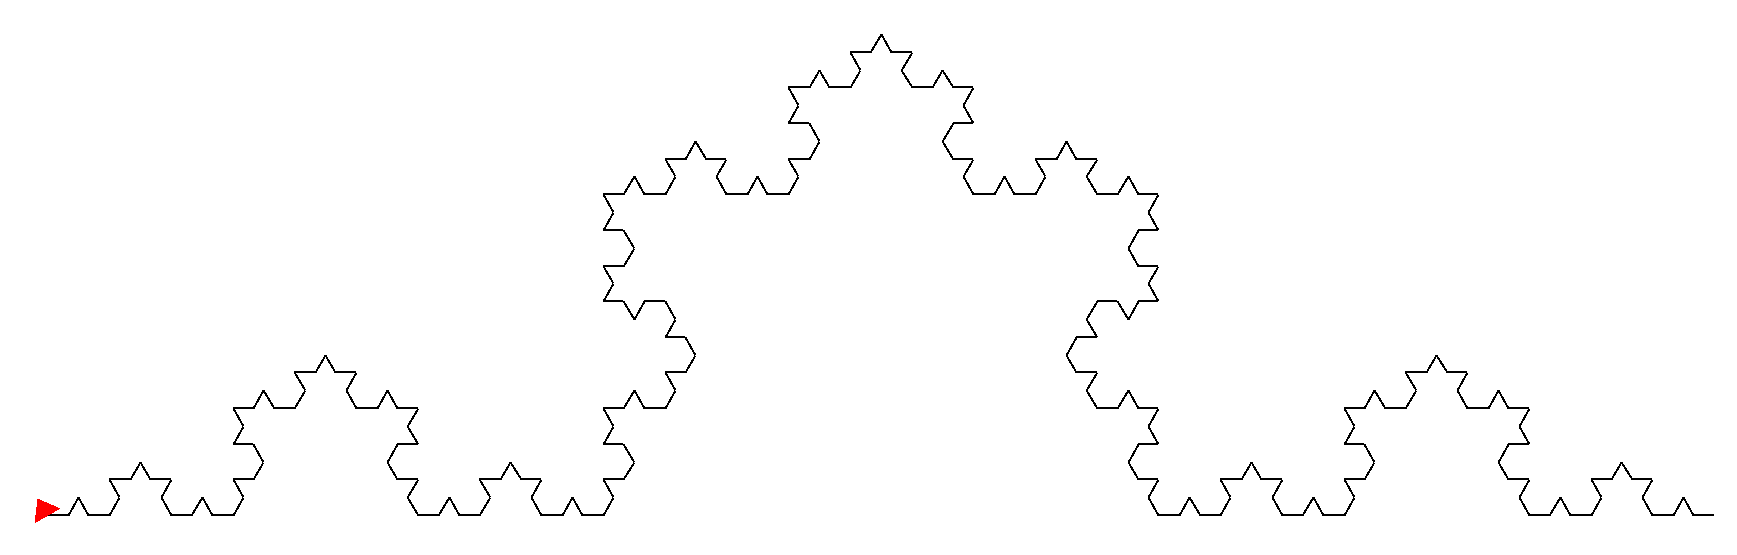
\includegraphics[width = \linewidth]{Thue-Morse Sequence/512.png}
		\caption{Iteration 4, $n=512$}
	\end{subfigure}
	\begin{subfigure}{0.3\linewidth}
		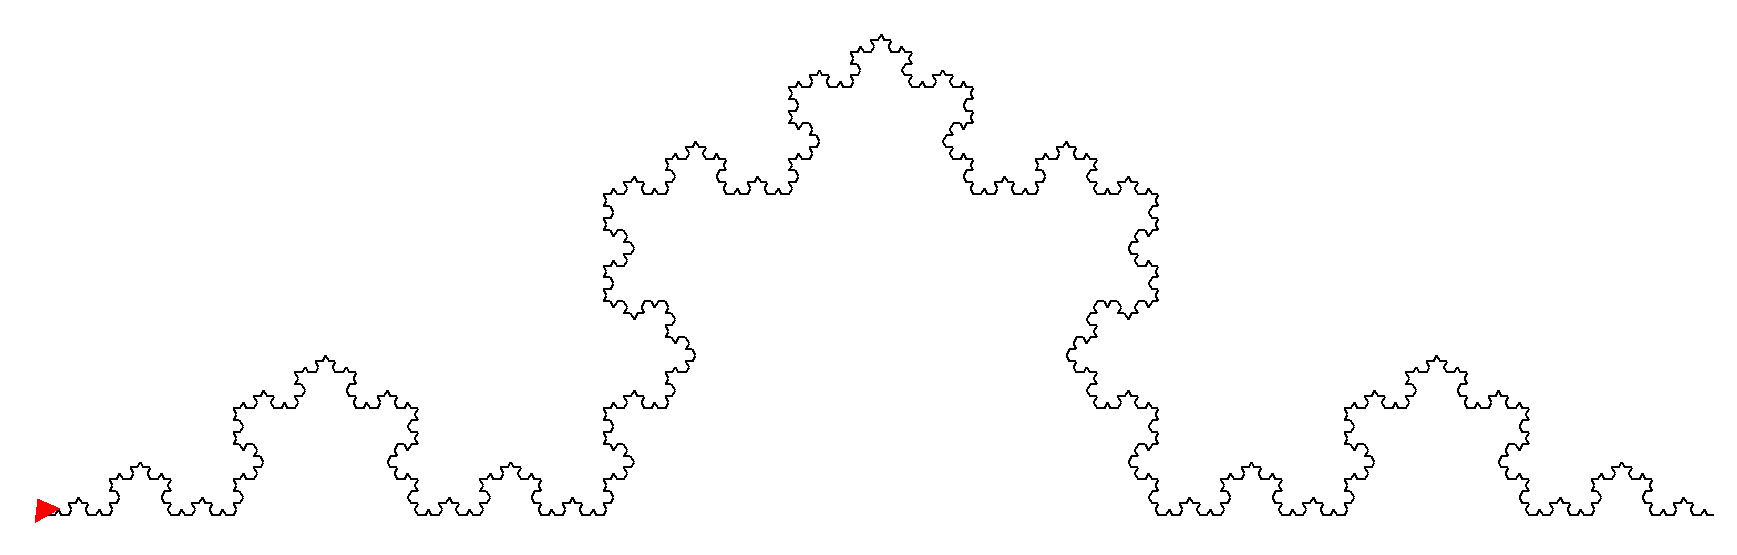
\includegraphics[width = \linewidth]{Thue-Morse Sequence/2048.png}
		\caption{Iteration 5, $n=2048$}
	\end{subfigure}
	\begin{subfigure}{0.3\linewidth}
		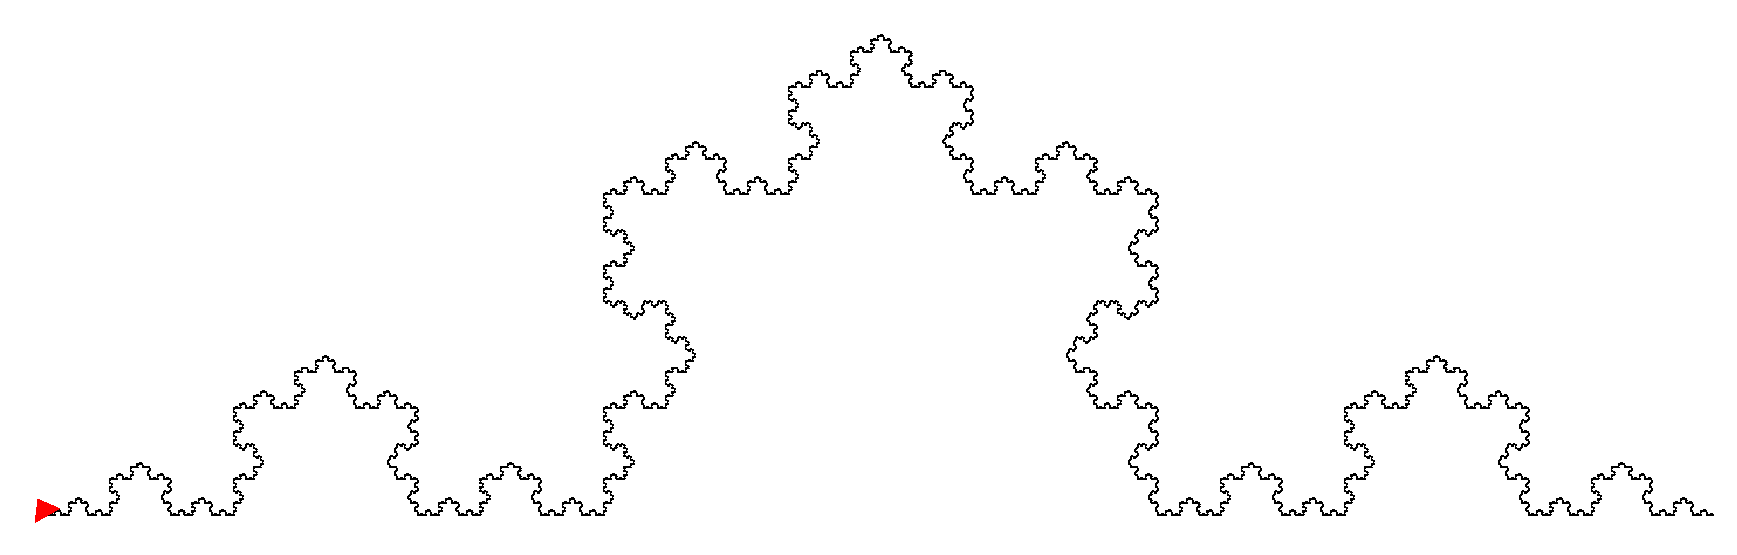
\includegraphics[width = \linewidth]{Thue-Morse Sequence/8192.png}
		\caption{Iteration 6, $n=8192$}
	\end{subfigure}
	\caption{Koch Curve Iterations and the outputs for odd powers of 2}
\end{figure}
\begin{figure}[H]
	\centering
	\begin{subfigure}{0.3\linewidth}
		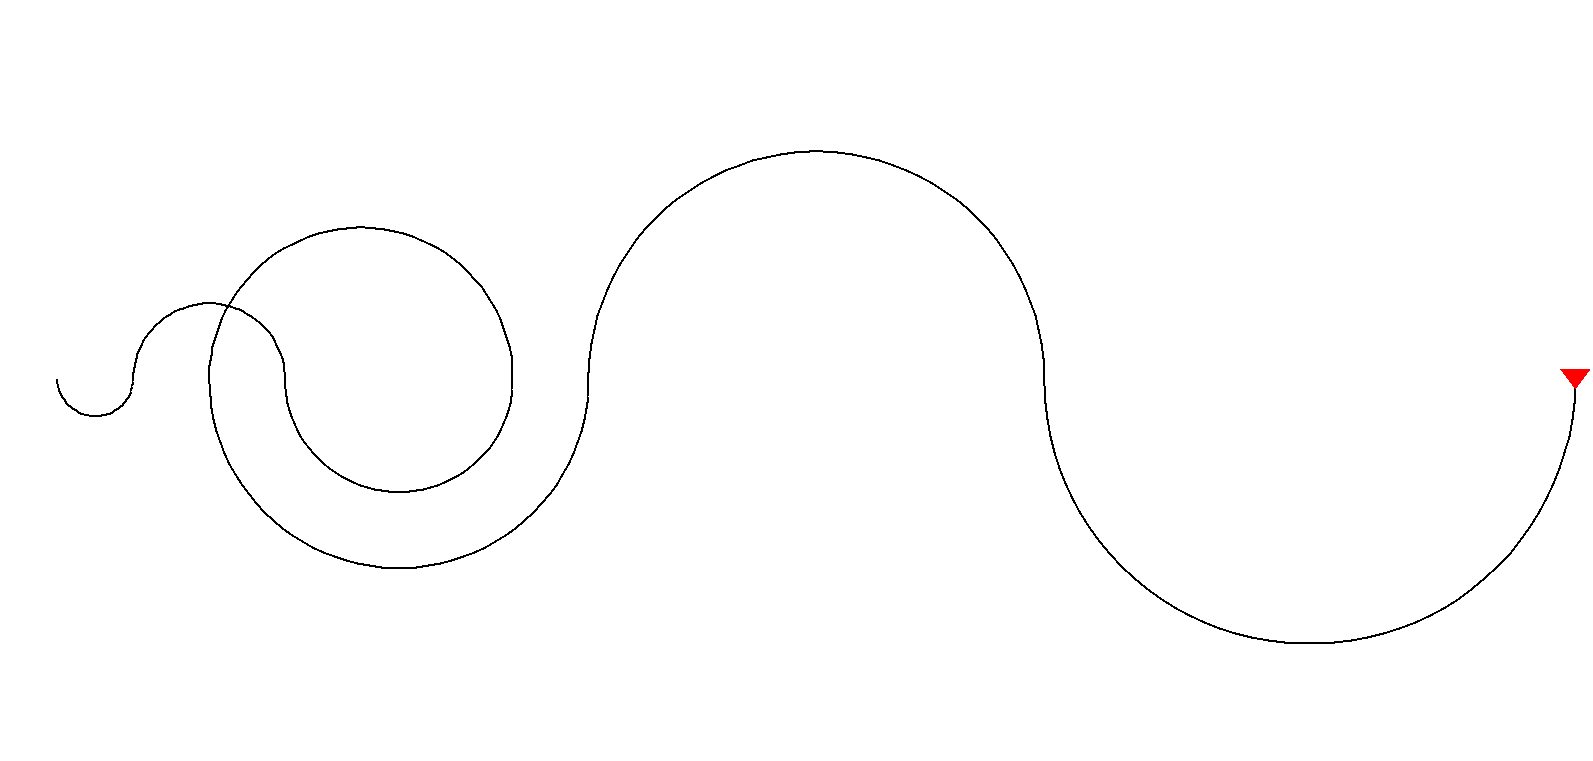
\includegraphics[width = \linewidth]{Thue-Morse Sequence/4.png}
		\caption{$n=4$}
	\end{subfigure}
	\begin{subfigure}{0.3\linewidth}
		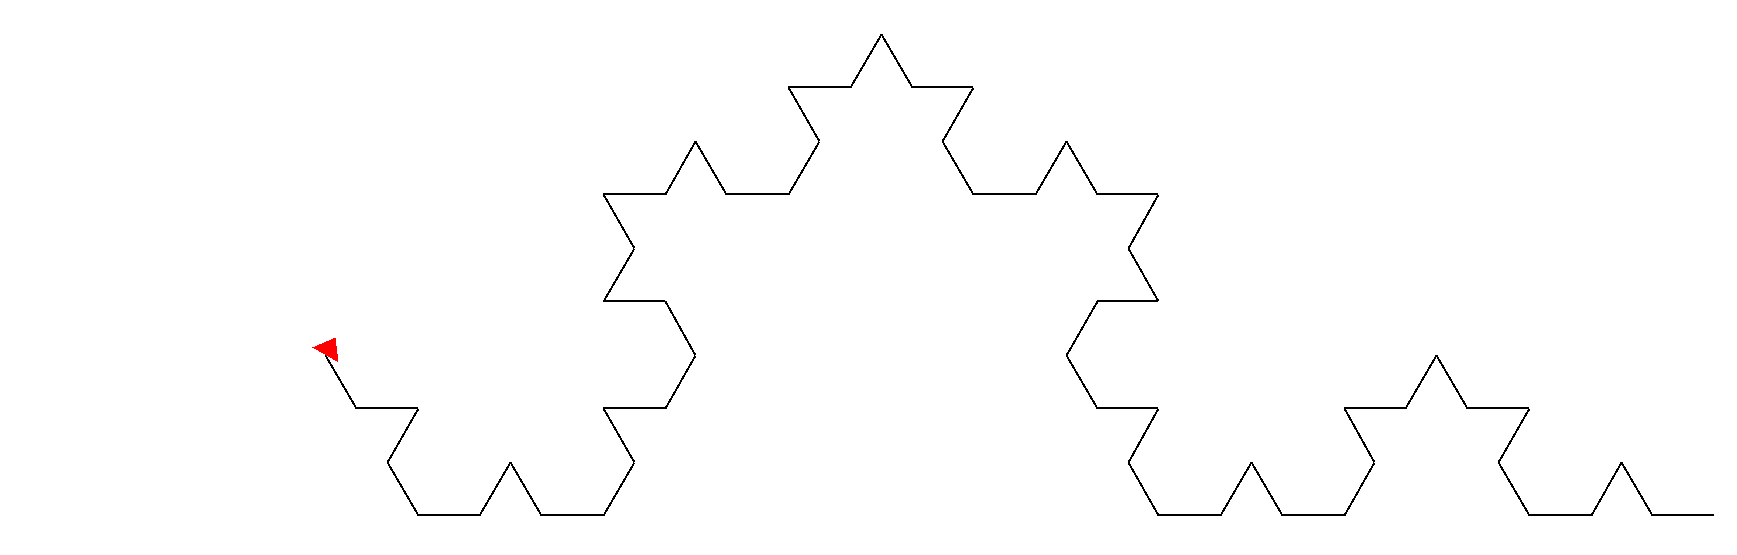
\includegraphics[width = \linewidth]{Thue-Morse Sequence/111.png}
		\caption{$n=111$}
	\end{subfigure}
	\begin{subfigure}{0.3\linewidth}
		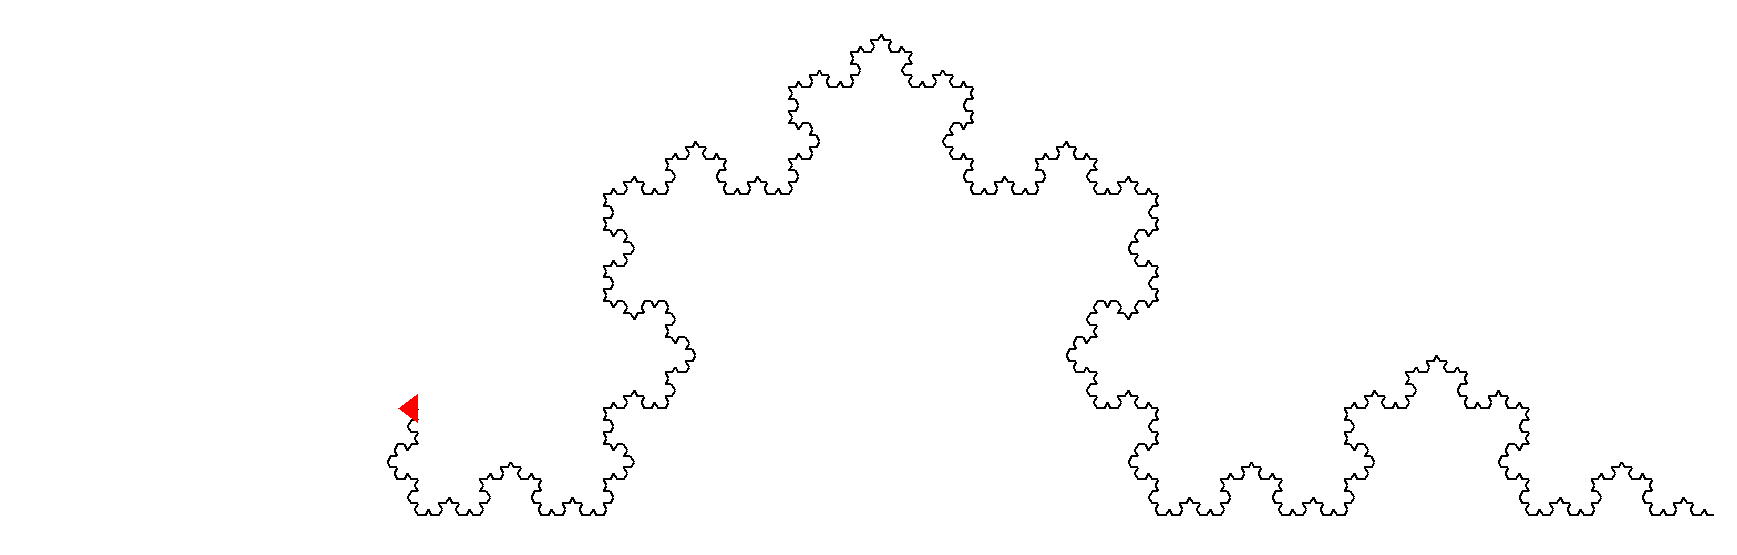
\includegraphics[width = \linewidth]{Thue-Morse Sequence/1729.png}
		\caption{$n=1729$}
	\end{subfigure}
	\caption{The outputs for non-odd powers of 2}
\end{figure}
\begin{funvideo}
	\href{https://youtu.be/prh72BLNjIk}{The Fairest Sharing Sequence Ever -- Stand-up Maths}\\
	\href{https://youtu.be/gB9n2gHsHN4}{Fractals are typically not self-similar -- 3Blue1Brown}
\end{funvideo}
\KOMAoptions{paper=A3}
\recalctypearea
\subsection{Linear Feedback Shift Register}
How does a computer generate truly random numbers? Computers are deterministic which means the actions it takes are predetermined. So it can’t generate truly random numbers unless they observe some unpredictable data like noise. But we can still generate “seemingly” random numbers called \textbf{pseudorandom numbers}. One such approach is using Linear Feedback Shift Registers (LFSRs).

An LFSR is defined by
\begin{itemize}	
	\item $n$ state variables $x_1, x_2, x_3,\ldots, x_n$ (collectively called as the state of LFSR (``register'')) with their initial values (called taps) $t_1, t_2, t_3,\ldots, t_n$ ($t_i$ is 0 or 1).
	\item A feedback polynomial $c_1x_0 + c_2x_1 + c_3x_2 + \cdots +  c_nx_{n-1} + x_n$ ($c_i$ is 0 or 1) which updates the state of LFSR as follows
	\begin{itemize}
		\item $\op{next}(x_1, x_2, x_3,\ldots, x_{n-1}) = (x_2, x_3, x_4,\ldots, x_n)$ -- this is called ``shifting'' next value of $x_1$ becomes $x_2$, next value of $x_2$ becomes $x_3$, and so on.
		\item $\op{next}(x_n) =  c_1x_1 \oplus c_2x_2 \oplus \cdots \oplus c_{n-1}x_{n-1}\oplus c_nx_n$ where $\oplus$ is the binary \href{https://en.wikipedia.org/wiki/Exclusive_or}{xor} operator -- this is the ``linear feedback''.
	\end{itemize}
	\item The output bit is $x_1$
\end{itemize}
For example, consider a $3-$bit LFSR as shown in \ref{fig:lfsrintro}. Here, $(t_1,t_2,t_3)=(1,1,0)$ and $(c_1,c_2,c_3)=(1,0,1)$.\\
Next, the sequence generation is shown in \ref{fig:lfsrgeneration}. Here, the initial state $(1,1,0)$ becomes $(1,0,1\oplus0) = (1,0,0)$ and with similar updates, eventually the sequence repeats when the state becomes $(1,1,1)$ as next state will be $(1,1,1\oplus1) = (1,1,0)$.
\begin{figure}[H]
	\centering
	\begin{subfigure}[c]{0.4\linewidth}
		\centering
		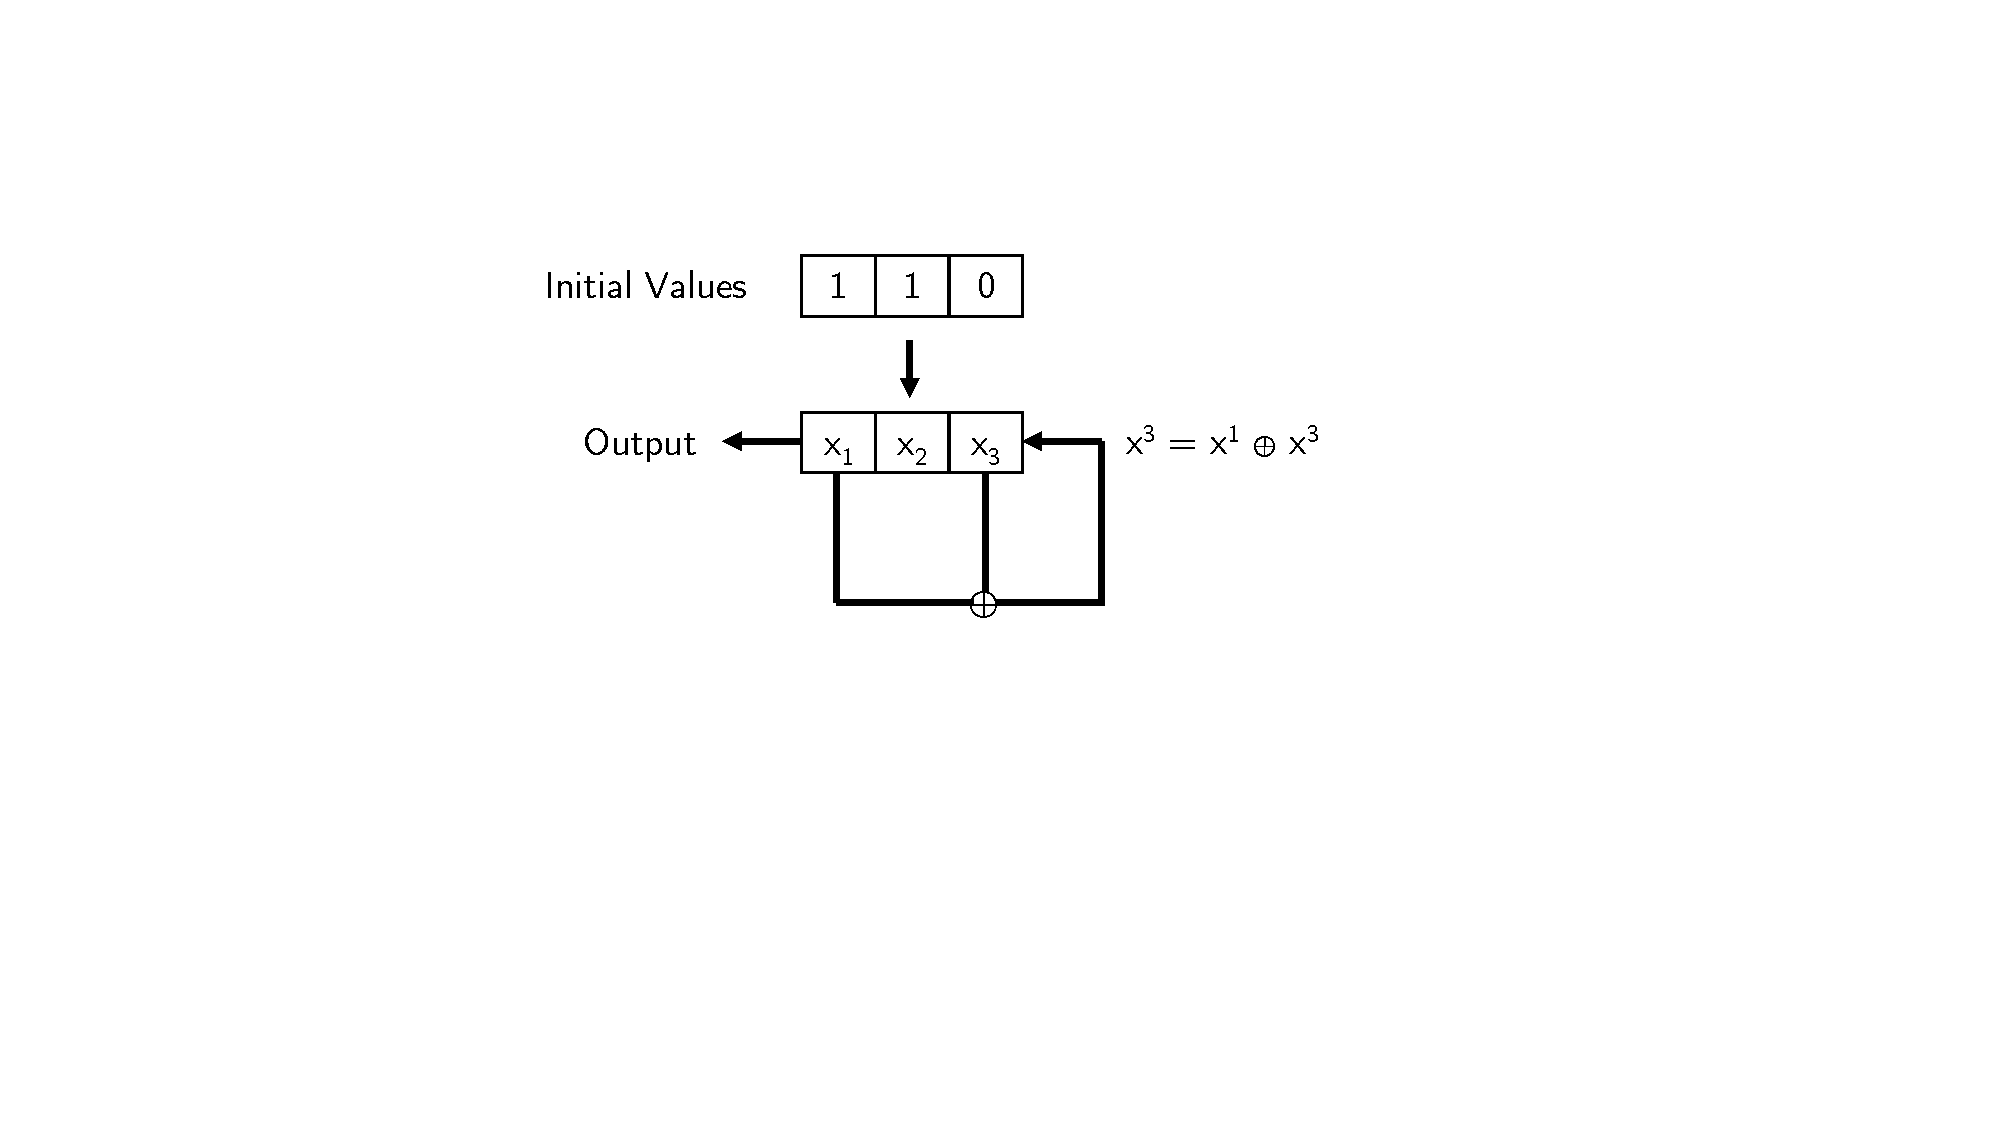
\includegraphics[width = \linewidth]{Linear Feedback Shift Register/Introduction.pdf}
		\caption{Given LFSR}
		\label{fig:lfsrintro}
	\end{subfigure}
	\begin{subfigure}[c]{0.45\linewidth}
		\centering
		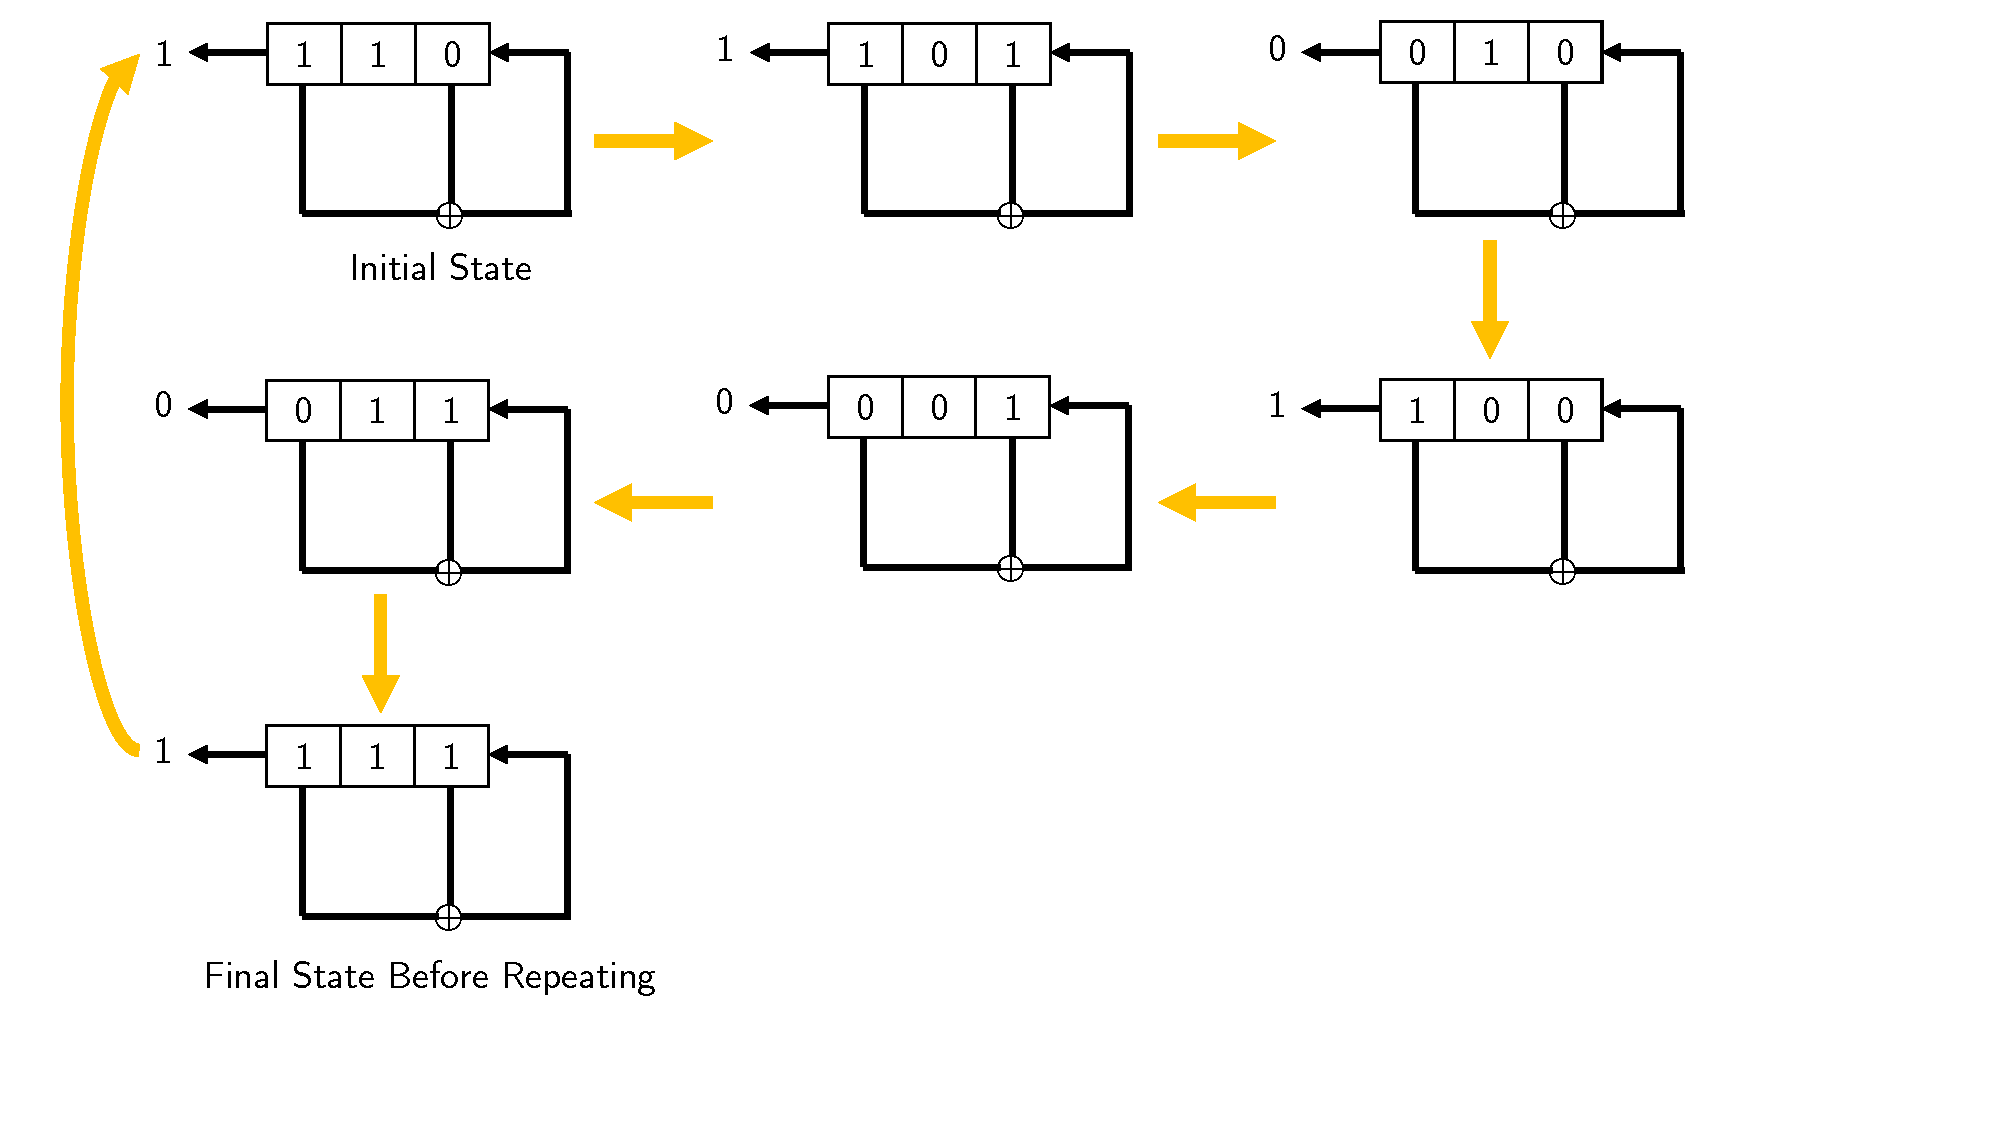
\includegraphics[width = \linewidth]{Linear Feedback Shift Register/Sequence Generation.pdf}
		\caption{The Generated Sequence is 11001001 repeating (follow the arrows)}
		\label{fig:lfsrgeneration}
	\end{subfigure}
	\caption{Linear Feedback Shift Register -- Working}
\end{figure}
\vspace{-2em}
\textbf{Problem Statement:}\\
A property of $n$ bit LFSR is that the output sequence it generates will start repeating in at most $2^{n-1}$ iterations called its period\footnote{Interestingly, there also exists a feedback polynomial which achieves this maximum period for every $n$.}.\\
Your task is to simulate an LFSR with a given initial state and feedback polynomial until it repeats and find its period\footnote{Is there a way to get the period of the sequence using just the feedback polynomial and without actually calculating sequence? The basis of this problem lie in the fascinating area of mathematics known as Abstract Algebra!
} in the process.
\begin{testcasesMore}
	{$t$ \hfill(number of test cases, an integer)\\
	$n_i\quad t_1\ t_2\ \cdots t_{n_i}\quad c_1\ c_2\ \cdots c_{n_i}$ \hfill($2n_i+1$ space seperated integers for each testcase)}
	{the output sequence generated by the given LFSR followed by the period of this output sequence\hfill(each iteration on a newline)}
	{$1 \leq n_i \leq 15$\\
	$t_i$ is either 0 or 1 and $c_1 = 1$\footnotemark,\ other $c_i$ are either 0 or 1\hfill(The LFSR will repeat from the beginning)}
	{1\quad 1 \quad 1\\2\quad1 0\quad1 0\\2 \quad 1 1 \quad 1 0\\2 \quad 1 1 \quad 1 1\\3 \quad 1 1 0 \quad 1 0 1\\5 \quad 1 0 1 0 0 \quad 1 0 0 1 0\\7 \quad 1 1 0 0 0 0 0 \quad 1 0 0 0 0 0 1}
	{1\quad1\\1 0\quad2\\1\quad1\\1 1 0\quad3\\1 1 0 1 0 0 1\quad7\\1 0 1 0 0 1 0 0 0 0 1 0 1 0 1 1 1 0 1 1 0 0 0 1 1 1 1 1 0 0 1\quad31\\1 1 0 0 0 0 0 1 0 0 0 0 0 0 1 1 1 1 1 1 1 0 1 0 1 0 1 0 0 1 1 0 0 1 1 1 0 1 1 1 0 1 0 0 1 0 1 1 0 0 0 1 1 0 1 1 1 1 0 1 1 0 1 0 1 1 0 1 1 0 0 1 0 0 1 0 0 0 1 1 1 0 0 0 0 1 0 1 1 1 1 1 0 0 1 0 1 0 1 1 1 0 0 1 1 0 1 0 0 0 1 0 0 1 1 1 1 0 0 0 1 0 1 0 0 0 0\quad127}
	{https://github.com/paramrathour/CS-101/tree/main/Test Cases/Linear Feedback Shift Register/Input.txt}
	{https://github.com/paramrathour/CS-101/tree/main/Test Cases/Linear Feedback Shift Register/Output.txt}
	{https://github.com/paramrathour/CS-101/tree/main/Starter Codes/Linear Feedback Shift Register.cpp}
\end{testcasesMore}
\footnotetext{This makes sure that the sequence will repeat from the beginning and will not have any non-periodic part. For example, $110101010\ldots$ (`10' repeating) is not possible if $c_1 = 1$.}
\begin{funvideo}
	\href{https://youtu.be/Ks1pw1X22y4}{Random Numbers with LFSR (Linear Feedback Shift Register) -- Computerphile}
\end{funvideo}
\KOMAoptions{paper=A4}
\recalctypearea